\documentclass[border=5pt]{standalone}
\usepackage{fontspec,unicode-math}
\setmainfont{Noto Serif}
\setmathfont{STIXTwoMath-Regular.otf}
\usepackage{tikz}
\usetikzlibrary{arrows.meta,calc,patterns,decorations.markings,decorations.pathmorphing}
\tikzset{lev/.style={line width=1.25pt,line cap=butt},
 fine/.style={line width=.60pt},band/.style={line width=.57pt},
 curve/.style={line width=1.35pt,line cap=round,line join=round},
 ax/.style={line width=.65pt,-{Latex[length=2.3mm,width=1.3mm]}},
 ray/.style={line width=.68pt,-{Latex[length=2.0mm,width=1.10mm]}},
 dimension/.style={line width=.57pt,{Latex[length=1.7mm,width=.9mm]}-{Latex[length=1.7mm,width=.9mm]}},
 flow/.style={line width=.68pt,postaction={decorate},decoration={markings,mark=at position .66 with {\arrow{Latex[length=2mm,width=1.1mm]}}}},
 lab/.style={font=\fontsize{13}{16}\selectfont,inner sep=1.3pt},
 small/.style={font=\fontsize{11}{13}\selectfont,inner sep=1.2pt},
 tinytext/.style={font=\fontsize{10}{12}\selectfont,inner sep=1pt},
 panel/.style={font=\fontsize{14}{16}\selectfont\itshape,inner sep=0pt}}
\pagestyle{empty}
\begin{document}
% CP14: singly/doubly ionized continua and 4 narrow intermediate states.
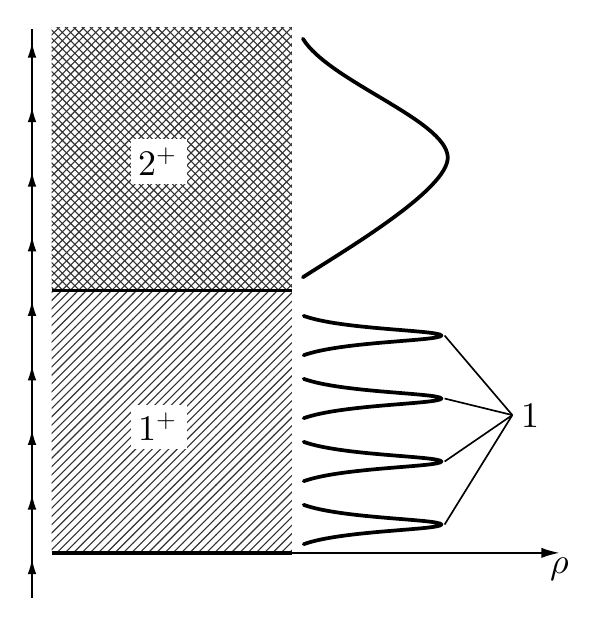
\begin{tikzpicture}[x=1cm,y=1cm,line join=round]
% Lower 1+ region and upper 2+ region; same density reference abscissa rho.
\path[pattern=north east lines,pattern color=black!80] (.80,.75) rectangle (3.85,4.08);
\path[pattern=crosshatch,pattern color=black!80] (.80,4.08) rectangle (3.85,7.42);
\draw[lev] (.80,.75)--(3.85,.75) (.80,4.08)--(3.85,4.08);
\node[lab,fill=white,inner sep=3pt] at (2.16,2.35) {$1^+$};
\node[lab,fill=white,inner sep=3pt] at (2.16,5.72) {$2^+$};
% Ascending multi-photon pathway: seven discrete arrowheads along the same ray.
\draw[fine] (.55,.18)--(.55,7.40);
\foreach \yy in {.50,1.32,2.14,2.96,3.78,4.60,5.42,6.24,7.06}{
 \draw[ray] (.55,\yy-.24)--(.55,\yy+.18);}
% Broad density maximum beyond second ionization threshold, not a discrete state.
\draw[curve] (3.99,7.28)
 .. controls (4.32,6.74) and (5.80,6.25) .. (5.83,5.78)
 .. controls (5.85,5.37) and (4.50,4.58) .. (3.99,4.25);
% Four *independent* narrow, long-lived one-electron autoionization resonances.
% Their vertical positions are schematic; 4 is author-drawn peak count.
\foreach \cent in {1.11,1.91,2.71,3.51}{
 \draw[curve] (4.00,\cent+.25)
  .. controls (4.48,\cent+.075) and (5.72,\cent+.070) .. (5.75,\cent)
  .. controls (5.72,\cent-.070) and (4.48,\cent-.075) .. (4.00,\cent-.25);}
% Four separately traceable pointers meet at the original callout '1'.
\foreach \cent in {1.11,1.91,2.71,3.51}{
 \draw[fine] (5.79,\cent)--(6.65,2.50);}
\node[lab,anchor=west] at (6.72,2.50) {$1$};
\draw[ax] (.8,.75)--(7.25,.75) node[lab,below] {$\rho$};
\end{tikzpicture}
\end{document}
